\documentclass{standalone}
\usepackage{tikz}
\usetikzlibrary{patterns, positioning}


\begin{document}
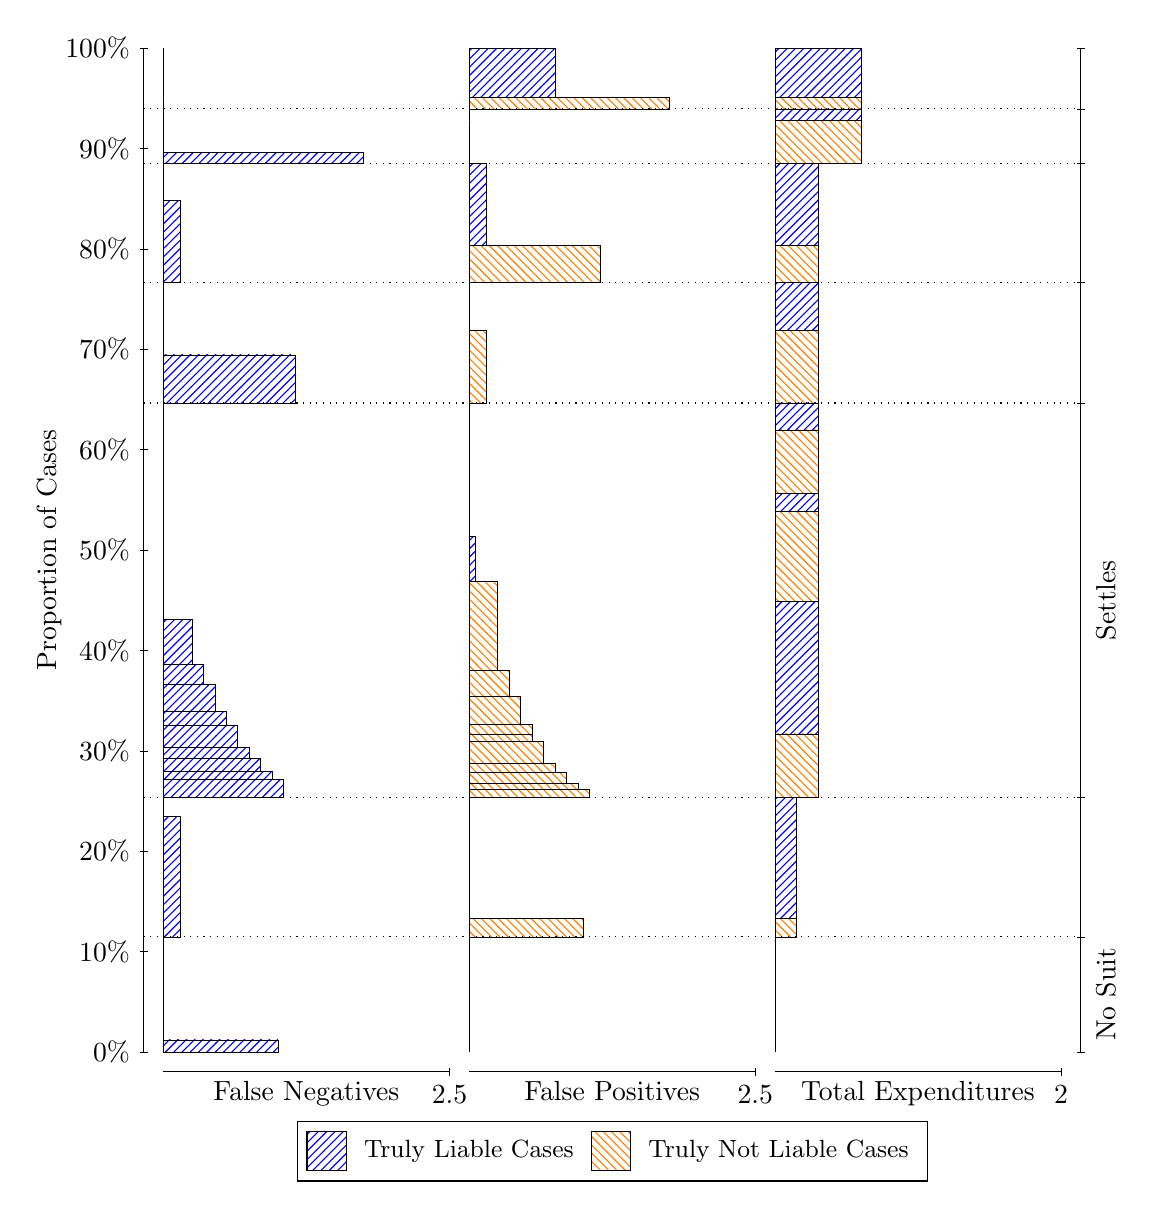
\begin{tikzpicture}
\draw[black, very thin] (1.5,1.75) -- (1.5,14.5);
\node[rotate=90, text=black, anchor=center] at (0.3, 8.125) {Proportion of Cases};
\draw[black, very thin] (1.45,1.75) -- (1.55,1.75);
\node[text=black, anchor=east] at (1.45, 1.75) {0\%};
\draw[black, very thin] (1.45,3.025) -- (1.55,3.025);
\node[text=black, anchor=east] at (1.45, 3.025) {10\%};
\draw[black, very thin] (1.45,4.3) -- (1.55,4.3);
\node[text=black, anchor=east] at (1.45, 4.3) {20\%};
\draw[black, very thin] (1.45,5.575) -- (1.55,5.575);
\node[text=black, anchor=east] at (1.45, 5.575) {30\%};
\draw[black, very thin] (1.45,6.85) -- (1.55,6.85);
\node[text=black, anchor=east] at (1.45, 6.85) {40\%};
\draw[black, very thin] (1.45,8.125) -- (1.55,8.125);
\node[text=black, anchor=east] at (1.45, 8.125) {50\%};
\draw[black, very thin] (1.45,9.4) -- (1.55,9.4);
\node[text=black, anchor=east] at (1.45, 9.4) {60\%};
\draw[black, very thin] (1.45,10.675) -- (1.55,10.675);
\node[text=black, anchor=east] at (1.45, 10.675) {70\%};
\draw[black, very thin] (1.45,11.95) -- (1.55,11.95);
\node[text=black, anchor=east] at (1.45, 11.95) {80\%};
\draw[black, very thin] (1.45,13.225) -- (1.55,13.225);
\node[text=black, anchor=east] at (1.45, 13.225) {90\%};
\draw[black, very thin] (1.45,14.5) -- (1.55,14.5);
\node[text=black, anchor=east] at (1.45, 14.5) {100\%};

\draw[black, very thin] (13.4,1.75) -- (13.4,14.5);
\draw[black, very thin] (13.35,1.75) -- (13.45,1.75);
\node[anchor=west] at (13.35, 1.75) {};
\draw[black, very thin] (13.35,3.2112) -- (13.45,3.2112);
\node[anchor=west] at (13.35, 3.2112) {};
\draw[black, very thin] (13.35,4.9802) -- (13.45,4.9802);
\node[anchor=west] at (13.35, 4.9802) {};
\draw[black, very thin] (13.35,9.9922) -- (13.45,9.9922);
\node[anchor=west] at (13.35, 9.9922) {};
\draw[black, very thin] (13.35,11.523) -- (13.45,11.523);
\node[anchor=west] at (13.35, 11.523) {};
\draw[black, very thin] (13.35,13.032) -- (13.45,13.032);
\node[anchor=west] at (13.35, 13.032) {};
\draw[black, very thin] (13.35,13.727) -- (13.45,13.727);
\node[anchor=west] at (13.35, 13.727) {};
\draw[black, very thin] (13.35,14.5) -- (13.45,14.5);
\node[anchor=west] at (13.35, 14.5) {};

\draw[black, very thin, pattern color=blue, pattern=north east lines] (1.75,1.75) rectangle (3.2033,1.9037);
\draw[black, very thin, pattern color=orange, pattern=north west lines] (1.75,1.9037) rectangle (1.75,3.2112);
\draw[black, very thin, pattern color=blue, pattern=north east lines] (1.75,3.2112) rectangle (1.968,4.7442);
\draw[black, very thin, pattern color=orange, pattern=north west lines] (1.75,4.7442) rectangle (1.75,4.9802);
\draw[black, very thin, pattern color=blue, pattern=north east lines] (1.75,4.9802) rectangle (3.276,5.2152);
\draw[black, very thin, pattern color=blue, pattern=north east lines] (1.75,5.2152) rectangle (3.1307,5.3135);
\draw[black, very thin, pattern color=blue, pattern=north east lines] (1.75,5.3135) rectangle (2.9853,5.4754);
\draw[black, very thin, pattern color=blue, pattern=north east lines] (1.75,5.4754) rectangle (2.84,5.6168);
\draw[black, very thin, pattern color=blue, pattern=north east lines] (1.75,5.6168) rectangle (2.6947,5.8976);
\draw[black, very thin, pattern color=blue, pattern=north east lines] (1.75,5.8976) rectangle (2.5493,6.0749);
\draw[black, very thin, pattern color=blue, pattern=north east lines] (1.75,6.0749) rectangle (2.404,6.4152);
\draw[black, very thin, pattern color=blue, pattern=north east lines] (1.75,6.4152) rectangle (2.2587,6.6745);
\draw[black, very thin, pattern color=blue, pattern=north east lines] (1.75,6.6745) rectangle (2.1133,7.2441);
\draw[black, very thin, pattern color=orange, pattern=north west lines] (1.75,7.2441) rectangle (1.75,9.9922);
\draw[black, very thin, pattern color=blue, pattern=north east lines] (1.75,9.9922) rectangle (3.4213,10.604);
\draw[black, very thin, pattern color=orange, pattern=north west lines] (1.75,10.604) rectangle (1.75,11.523);
\draw[black, very thin, pattern color=blue, pattern=north east lines] (1.75,11.523) rectangle (1.968,12.563);
\draw[black, very thin, pattern color=orange, pattern=north west lines] (1.75,12.563) rectangle (1.75,13.032);
\draw[black, very thin, pattern color=blue, pattern=north east lines] (1.75,13.032) rectangle (4.2933,13.178);
\draw[black, very thin, pattern color=orange, pattern=north west lines] (1.75,13.178) rectangle (1.75,13.727);
\draw[black, very thin, pattern color=orange, pattern=north west lines] (1.75,13.727) rectangle (1.75,13.873);
\draw[black, very thin, pattern color=blue, pattern=north east lines] (1.75,13.873) rectangle (1.75,14.5);
\draw[black, very thin, pattern color=orange, pattern=north west lines] (5.6333,1.75) rectangle (5.6333,3.0574);
\draw[black, very thin, pattern color=blue, pattern=north east lines] (5.6333,3.0574) rectangle (5.6333,3.2112);
\draw[black, very thin, pattern color=orange, pattern=north west lines] (5.6333,3.2112) rectangle (7.0867,3.4471);
\draw[black, very thin, pattern color=blue, pattern=north east lines] (5.6333,3.4471) rectangle (5.6333,4.9802);
\draw[black, very thin, pattern color=orange, pattern=north west lines] (5.6333,4.9802) rectangle (7.1593,5.0821);
\draw[black, very thin, pattern color=orange, pattern=north west lines] (5.6333,5.0821) rectangle (7.014,5.1655);
\draw[black, very thin, pattern color=orange, pattern=north west lines] (5.6333,5.1655) rectangle (6.8687,5.3038);
\draw[black, very thin, pattern color=orange, pattern=north west lines] (5.6333,5.3038) rectangle (6.7233,5.4163);
\draw[black, very thin, pattern color=orange, pattern=north west lines] (5.6333,5.4163) rectangle (6.578,5.6985);
\draw[black, very thin, pattern color=orange, pattern=north west lines] (5.6333,5.6985) rectangle (6.4327,5.7887);
\draw[black, very thin, pattern color=orange, pattern=north west lines] (5.6333,5.7887) rectangle (6.4327,5.9093);
\draw[black, very thin, pattern color=orange, pattern=north west lines] (5.6333,5.9093) rectangle (6.2873,6.2663);
\draw[black, very thin, pattern color=orange, pattern=north west lines] (5.6333,6.2663) rectangle (6.142,6.5918);
\draw[black, very thin, pattern color=orange, pattern=north west lines] (5.6333,6.5918) rectangle (5.9967,7.7283);
\draw[black, very thin, pattern color=blue, pattern=north east lines] (5.6333,7.7283) rectangle (5.706,8.2979);
\draw[black, very thin, pattern color=blue, pattern=north east lines] (5.6333,8.2979) rectangle (5.6333,9.9922);
\draw[black, very thin, pattern color=orange, pattern=north west lines] (5.6333,9.9922) rectangle (5.8513,10.911);
\draw[black, very thin, pattern color=blue, pattern=north east lines] (5.6333,10.911) rectangle (5.6333,11.523);
\draw[black, very thin, pattern color=orange, pattern=north west lines] (5.6333,11.523) rectangle (7.3047,11.992);
\draw[black, very thin, pattern color=blue, pattern=north east lines] (5.6333,11.992) rectangle (5.8513,13.032);
\draw[black, very thin, pattern color=orange, pattern=north west lines] (5.6333,13.032) rectangle (5.6333,13.58);
\draw[black, very thin, pattern color=blue, pattern=north east lines] (5.6333,13.58) rectangle (5.6333,13.727);
\draw[black, very thin, pattern color=orange, pattern=north west lines] (5.6333,13.727) rectangle (8.1767,13.873);
\draw[black, very thin, pattern color=blue, pattern=north east lines] (5.6333,13.873) rectangle (6.7233,14.5);
\draw[black, very thin, pattern color=orange, pattern=north west lines] (9.5167,1.75) rectangle (9.5167,3.0574);
\draw[black, very thin, pattern color=blue, pattern=north east lines] (9.5167,3.0574) rectangle (9.5167,3.2112);
\draw[black, very thin, pattern color=orange, pattern=north west lines] (9.5167,3.2112) rectangle (9.7892,3.4471);
\draw[black, very thin, pattern color=blue, pattern=north east lines] (9.5167,3.4471) rectangle (9.7892,4.9802);
\draw[black, very thin, pattern color=orange, pattern=north west lines] (9.5167,4.9802) rectangle (10.062,5.7887);
\draw[black, very thin, pattern color=blue, pattern=north east lines] (9.5167,5.7887) rectangle (10.062,7.4754);
\draw[black, very thin, pattern color=orange, pattern=north west lines] (9.5167,7.4754) rectangle (10.062,8.6119);
\draw[black, very thin, pattern color=blue, pattern=north east lines] (9.5167,8.6119) rectangle (10.062,8.8469);
\draw[black, very thin, pattern color=orange, pattern=north west lines] (9.5167,8.8469) rectangle (10.062,9.6499);
\draw[black, very thin, pattern color=blue, pattern=north east lines] (9.5167,9.6499) rectangle (10.062,9.9922);
\draw[black, very thin, pattern color=orange, pattern=north west lines] (9.5167,9.9922) rectangle (10.062,10.911);
\draw[black, very thin, pattern color=blue, pattern=north east lines] (9.5167,10.911) rectangle (10.062,11.523);
\draw[black, very thin, pattern color=orange, pattern=north west lines] (9.5167,11.523) rectangle (10.062,11.992);
\draw[black, very thin, pattern color=blue, pattern=north east lines] (9.5167,11.992) rectangle (10.062,13.032);
\draw[black, very thin, pattern color=orange, pattern=north west lines] (9.5167,13.032) rectangle (10.607,13.58);
\draw[black, very thin, pattern color=blue, pattern=north east lines] (9.5167,13.58) rectangle (10.607,13.727);
\draw[black, very thin, pattern color=orange, pattern=north west lines] (9.5167,13.727) rectangle (10.607,13.873);
\draw[black, very thin, pattern color=blue, pattern=north east lines] (9.5167,13.873) rectangle (10.607,14.5);
\draw[black, dotted] (1.5,3.2112) -- (13.4,3.2112);
\draw[black, dotted] (1.5,4.9802) -- (13.4,4.9802);
\draw[black, dotted] (1.5,9.9922) -- (13.4,9.9922);
\draw[black, dotted] (1.5,11.523) -- (13.4,11.523);
\draw[black, dotted] (1.5,13.032) -- (13.4,13.032);
\draw[black, dotted] (1.5,13.727) -- (13.4,13.727);
\draw[black, very thin] (1.75,1.5) -- (5.3833,1.5);
\node[text=black, anchor=north] at (3.5667, 1.5) {False Negatives};
\draw[black, very thin] (5.3833,1.45) -- (5.3833,1.55);
\node[text=black, anchor=north] at (5.3833, 1.45) {2.5};

\draw[black, very thin] (5.6333,1.5) -- (9.2667,1.5);
\node[text=black, anchor=north] at (7.45, 1.5) {False Positives};
\draw[black, very thin] (9.2667,1.45) -- (9.2667,1.55);
\node[text=black, anchor=north] at (9.2667, 1.45) {2.5};

\draw[black, very thin] (9.5167,1.5) -- (13.15,1.5);
\node[text=black, anchor=north] at (11.333, 1.5) {Total Expenditures};
\draw[black, very thin] (13.15,1.45) -- (13.15,1.55);
\node[text=black, anchor=north] at (13.15, 1.45) {2};

\node[text=black, centered, rotate=90] at (13.72, 2.4806) {No Suit};

\node[text=black, centered, rotate=90] at (13.72, 7.4862) {Settles};





\draw (7.449999999999999,1.5) node[draw=none] (baseCoordinate) {};
\begin{scope}[align=center]
        \matrix[scale=0.5, draw=black, below=0.5cm of baseCoordinate, nodes={draw}, column sep=0.1cm]{
            \node[rectangle, draw, minimum width=0.5cm, minimum height=0.5cm, pattern color=blue, pattern=north east lines] {}; &
            \node[draw=none, font=\small, text=black] (B) {Truly Liable Cases}; &
            \node[rectangle, draw, minimum width=0.5cm, minimum height=0.5cm, pattern color=orange, pattern=north west lines] {}; &
            \node[draw=none, font=\small, text=black] (B) {Truly Not Liable Cases}; \\
            };
\end{scope}

\end{tikzpicture}
\end{document}